%struts2
\section{Struts2}
\subsection{开发环境的搭建}
\subsubsection{所需的jar包}
\begin{description}
\item[struts-core-2.x.x.jar]	Struts2框架的核心类库
\item[xwork-2.x.x.jar]	XWork类库,Struts 2在其上构建
\item[ognl-2.6.x.jar]	对象图导航语言,struts2框架通过其读写对象的属性
\item[freemarker-2.3.x.jar]	Struts2的UI标签的模板使用FreeMarker编写
\item[commons-logging-1.1.x.jar]	ASF出品的日志包,Struts2框架使用这个日志包来支持Log4j和JDK1.4+的日志记录
\item[commons-fileupload-1.2.1.jar]	文件上传组件,2.1.6版本后必须加入此文件  
\end{description}

\subsubsection{编写配置文件struts.xml}
\begin{lstlisting}[style=JAVA]
<?xml version="1.0" encoding="UTF-8" ?>
<!DOCTYPE struts PUBLIC "-//Apache Software Foundation//DTD Struts Configuration 2.1//EN" "http://struts.apache.org/dtds/struts-2.1.dtd">
<struts>
	<package name="myactions" namespace="/"
		extends="struts-default">
		<action name="login" class="com.cm.LoginAction">
			<result name="success">/success.jsp</result>
			<result name="error">/error.jsp</result>
		</action>
	</package>
</struts>    
\end{lstlisting}
\begin{itemize}
\item package属性说明
\begin{description}
\item[name]	与java里面的包功能类似,将相同功能的action放在一个包里,易于管理
\item[namespace]	namespace作为action中访问路径path属性的一部分,可以简化代码
\item[extend]	默认继承struts-default包--Struts2很多核心的功能都是拦截器来实现的,
不继承struts-default就无法使用struts2提供的核心功能
\end{description}


\item action属性说明
\begin{description}
\item[name]	action名称,也可作为action路径的一部分.可以用通配符*,用来执行不同的方法
\item[class]	处理的类,默认的是ActionSupport
\item[method]	默认的是execute方法来执行
\item[result]	视图部分,用来导向x.jsp文件
\item[param]		通过struts.xml传递参数给action类(用set方法接受),然后进行处理
\end{description}
\begin{lstlisting}[style=JAVA]
<struts>
	<package name="myactions" namespace="/"
		extends="struts-default">
		<action name="login_*" class="com.cm.LoginAction" method="{1}">
			<result name="success">/success.jsp</result>
		</action>
	</package>
</struts>    
\end{lstlisting}
若访问的action名为login\_{}addUI,这会匹配该action,并执行addUI方法.


\item 常用常量
\begin{description}
\item[struts.action.extension]	设定访问action文件时用的后缀名
\begin{lstlisting}[style=JAVA]
<struts>
	<constant name="struts.action.extension" value="do,action"/>
</struts>    
\end{lstlisting}

\item[struts.i18n.encoding] 指定默认编码集,作用于HttpServletRequest的\\
setCharacterEncoding和freemarker,velovity的输出
\begin{lstlisting}[style=JAVA]
<struts>
	<constant name="struts.i18n.encoding" value="UTF-8"/>
</struts>    
\end{lstlisting}

\item[struts.configuration.xml.reload]	当struts.xml文件修改后,系统自动重新加载改文件,
默认值为false,开发阶段最好打开
\begin{lstlisting}[style=JAVA]
<struts>
	<constant name="struts.configuration.xml.reload" value="true"/>
</struts>    
\end{lstlisting}

\item[struts.ui.theme]	使用默认的视图主题,值为simple时在使用JSTL标签时不会生成额外代码
\begin{lstlisting}[style=JAVA]
<struts>
	<constant name="struts.ui.theme" value="simple"></constant>
</struts>    
\end{lstlisting}

\item[struts.enable.DynamicMethodInvocation]	设置struts2是否允许使用动态方法调用
\begin{lstlisting}[style=JAVA]
<struts>
	<constant name="struts.enable.DynamicMethodInvocation" value="false"/>
</struts>    
\end{lstlisting}

\item[struts.multipart.maxSize] 设置struts2能上传文件的大小限制
\begin{lstlisting}[style=JAVA]
<struts>
	<constant name="struts.multipart.maxSize" value="10701096"/>
</struts>    
\end{lstlisting}
\end{description}

\item 多个配置文件\\
当系统中action数量大量增加后,会导致struts.xml配置文件变得非常臃肿.为提高struts.xml文件的
可读性,可以将一个struts.xml配置文件分解成多个配置文件,然后在struts.xml中包含其他配置文件即可.
\begin{lstlisting}[style=JAVA]
<struts>
	<include file="struts-user.xml"/>
	<include file="struts-order.xml"/>
</struts>    
\end{lstlisting}


\end{itemize}

\subsubsection{添加StrutsMVC框架启动配置}
\begin{lstlisting}[style=JAVA]
<?xml version="1.0" encoding="UTF-8"?>
<web-app version="3.0" 
	xmlns="http://java.sun.com/xml/ns/javaee" 
	xmlns:xsi="http://www.w3.org/2001/XMLSchema-instance" 
	xsi:schemaLocation="http://java.sun.com/xml/ns/javaee 
	http://java.sun.com/xml/ns/javaee/web-app_3_0.xsd">
	
  <display-name></display-name>	
  
  <welcome-file-list>
    <welcome-file>index.jsp</welcome-file>
  </welcome-file-list>
  
  <filter>
  	<filter-name>struts2</filter-name>
  	<filter-class>
  		org.apache.struts2.dispatcher.ng.filter.StrutsPrepareAndExecuteFilter
  	</filter-class>
  </filter>
  
  <filter-mapping>
  	<filter-name>struts2</filter-name>
  	<url-pattern>/*</url-pattern>
  </filter-mapping></web-app>
\end{lstlisting}
注:\underline{自从Sturts2.1.3以后,org.apache.struts2.FilterDispatcher已经标注为过时了.}


\subsection{struts2的处理流程}
流程如下图\ref{figs2:fig1}所示:
\begin{figure}[!htbp]
	\centering
	\caption{struts2的工作流程}
    	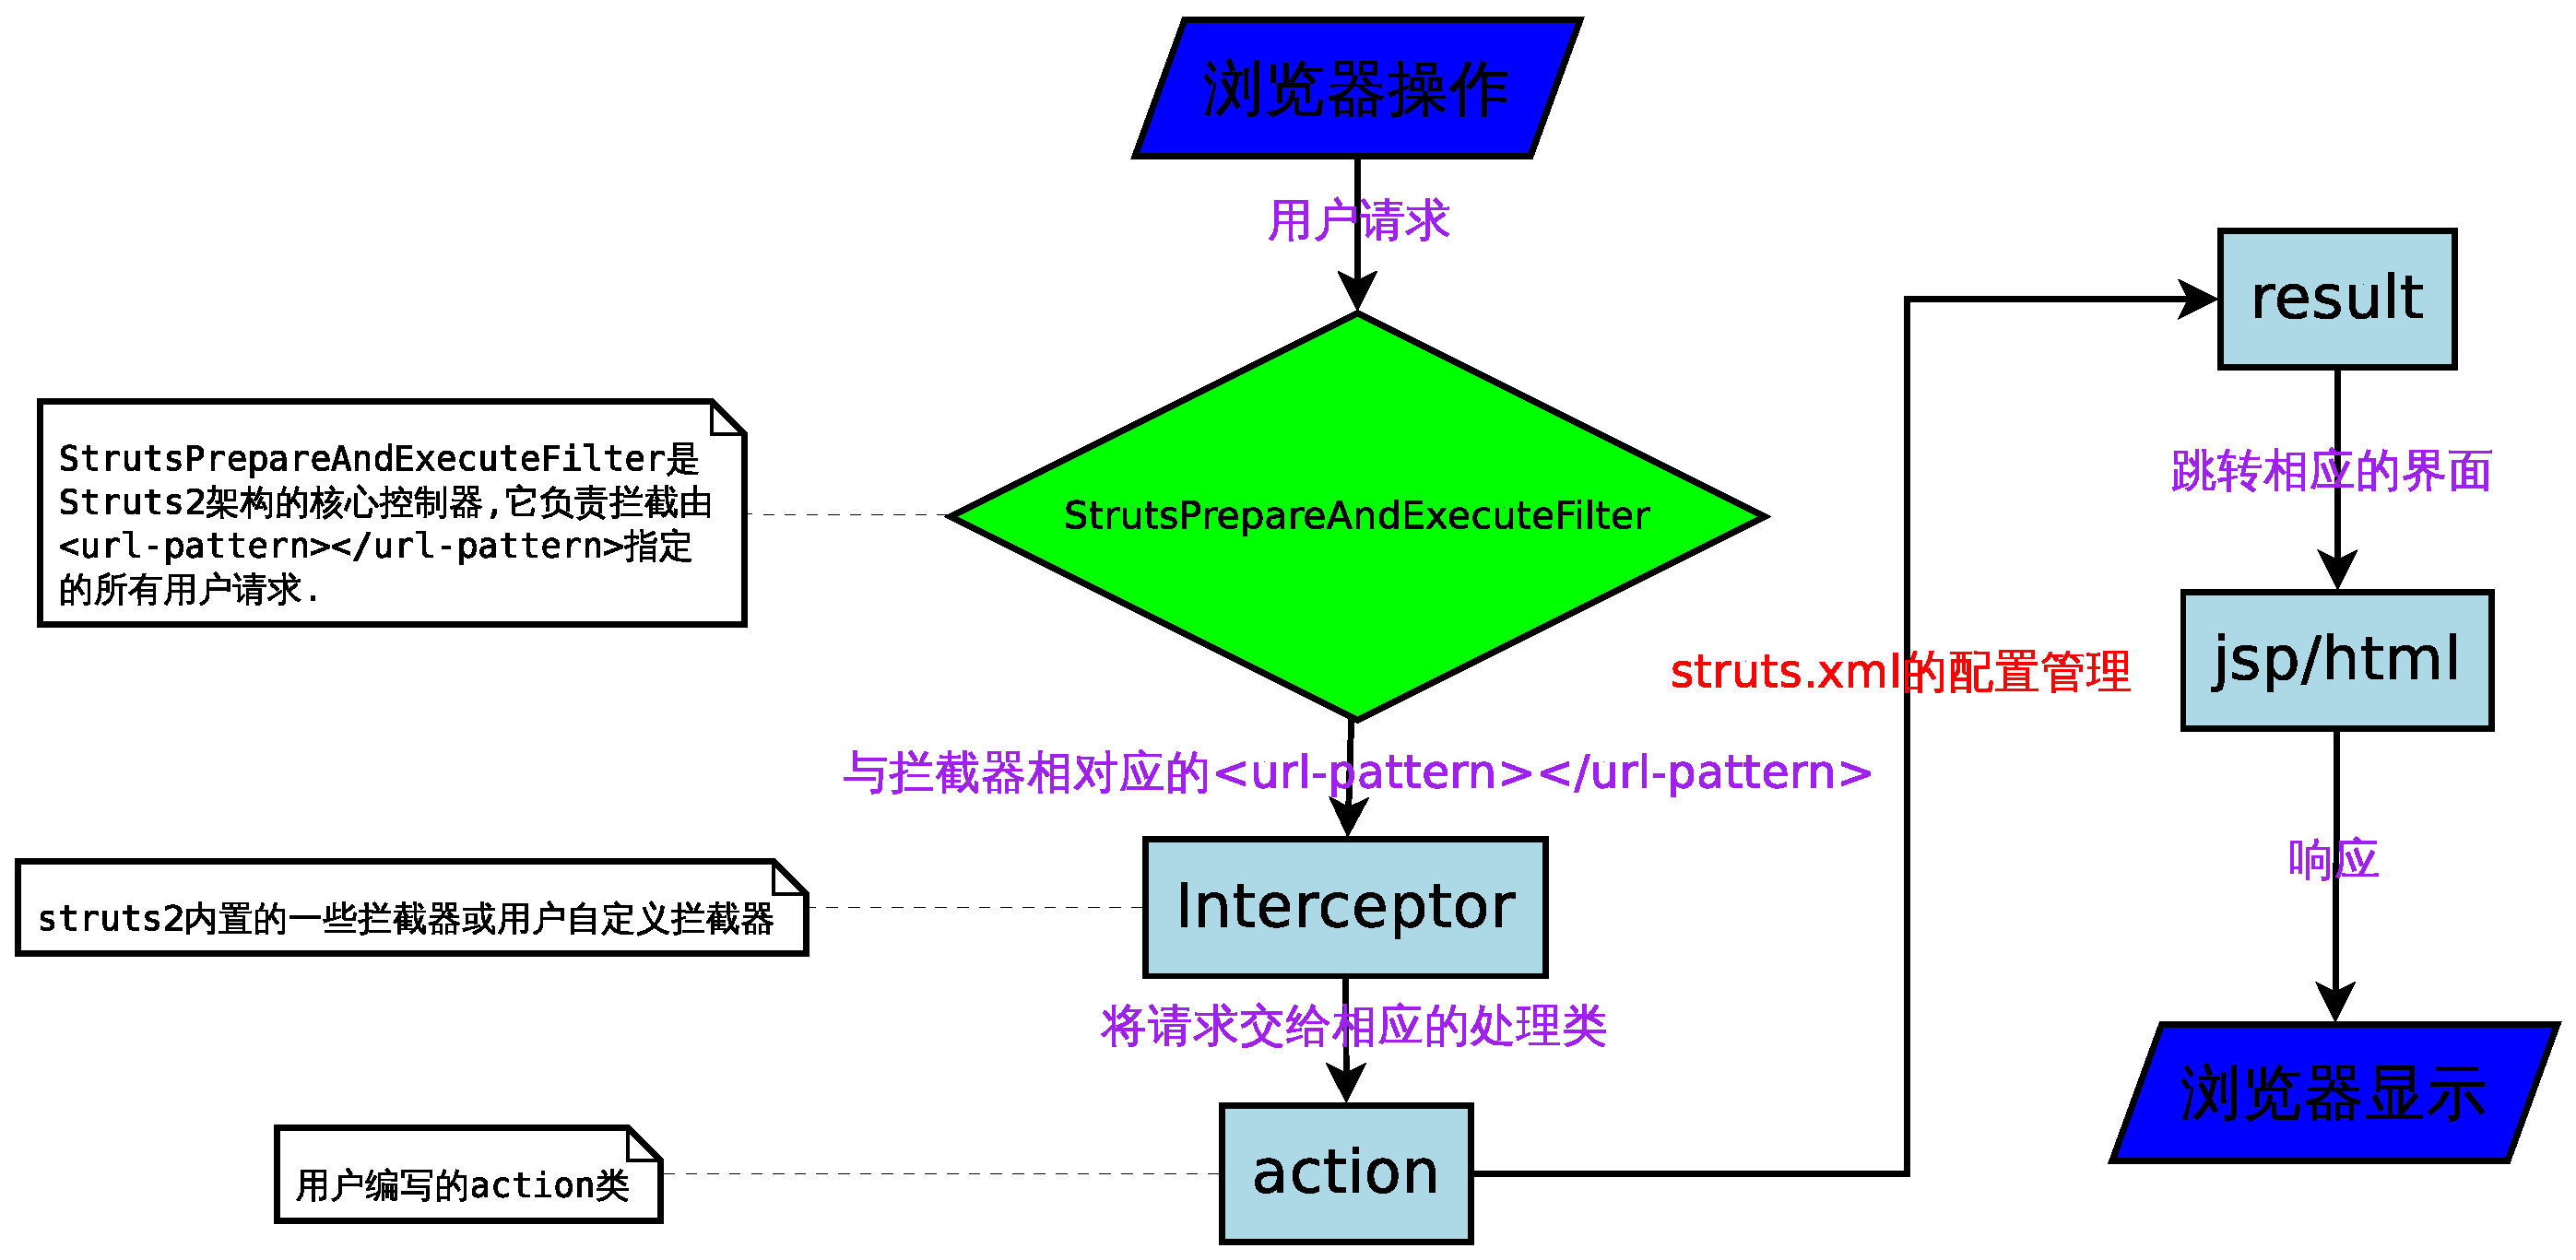
\includegraphics[scale=0.25]{figs/STRUTS2}
    \label{figs2:fig1}
\end{figure}


\subsection{struts2中的session/application/request}
\subsubsection{一般用法}
\begin{lstlisting}[style=JAVA]
public String execute() {
	//usage--only to access the attributes of the three objects
	ActionContext ctx = ActionContext.getContext();
	ctx.getApplication().put("app", "应用范围");	//put app into ServletContext
	ctx.getSession().put("ses", "session范围");	//put ses into session
	ctx.put("req", "request范围");				//put req into request
	ctx.put("names", Arrays.asList("老王","老张","老徐"));
	return "mySession";
}
\end{lstlisting}

\subsubsection{另一种用法}
\begin{lstlisting}[style=JAVA]
//access it directly by class--ServletActionContext
public String rsa() throws Exception{
	//usage--get the real path(servletContext.getRealPath) of the website
	HttpServletRequest request = ServletActionContext.getRequest();
	ServletContext servletContext = ServletActionContext.getServletContext();
	request.setAttribute("req", "请求范围属性");
	request.getSession().setAttribute("ses", "会话范围属性");
	servletContext.setAttribute("app", "应用范围属性");
	//HttpServletResponse response = ServletActionContext.getResponse();
	return "mySession";
}
\end{lstlisting}


\subsection{文件上传}
\subsubsection{所需的jar包}
在WEB-INF/lib下加入下面的jar包
\begin{enumerate}
\item commons-fileupload-1.2.1.jar
\item commons-io-1.3.2.jar
\end{enumerate}

\subsubsection{设置form表的enctype}
将form表的enctype设置为"multipart/form-data"
\begin{lstlisting}[style=JAVA]
//access it directly by class--ServletActionContext
public String rsa() throws Exception{
	//usage--get the real path(servletContext.getRealPath) of the website
	HttpServletRequest request = ServletActionContext.getRequest();
	ServletContext servletContext = ServletActionContext.getServletContext();
	request.setAttribute("req", "请求范围属性");
	request.getSession().setAttribute("ses", "会话范围属性");
	servletContext.setAttribute("app", "应用范围属性");
	//HttpServletResponse response = ServletActionContext.getResponse();
	return "mySession";
}
\end{lstlisting}



\subsection{struts2中的拦截器}
\subsubsection{类型转换器}
\begin{itemize}
\item 局部类型转换器	只对某个action起作用
\begin{enumerate}
\item 自定义类型转换器
\begin{lstlisting}[style=JAVA]
package com.hjy.type.converter;

import java.sql.Date;
import java.text.ParseException;
import java.text.SimpleDateFormat;
import java.util.Map;

import com.opensymphony.xwork2.conversion.impl.DefaultTypeConverter;

public class DateTypeConverter extends DefaultTypeConverter {

	@Override
	public Object convertValue(Map<String, Object> context, Object value,
			Class toType) {
		// TODO Auto-generated method stub
		SimpleDateFormat dateFormat = new SimpleDateFormat("yyyyMMdd");
		try{
			if(toType == Date.class){					//String--Date
				String[] params = (String[]) value;		//requese.getParameterValues()--all parameters
				return dateFormat.parse(params[0]);
			}else if(toType ==String.class){			//Date--String
				Date date = (Date) value;
				return dateFormat.format(date);
			}
		}catch(ParseException e){
			return null;
		}
		return super.convertValue(context, value, toType);
	}
}
\end{lstlisting}

\item 注册局部类型转换器
在\textcolor{red}{Action类}所在的包下放置\textcolor{red}{ActionClassName}-conversion.properties文件,
ActionClassName是Action的类名,后面的-conversion.properties是固定写法.在properties文件中的内容为
\textbf{\textcolor{red}{属性名称}=类型转换器的全类名}.
\end{enumerate}

\item 全局类型转换器	对整个应用都起作用
\begin{enumerate}
\item 自定义类型转换器\\
方法见局部类型转换器.


\item 注册全局类型转换器
在\textcolor{red}{src}所在的包下放置\textcolor{red}{xwork}-conversion.properties文件,后面的
-conversion.properties是固定写法.在properties文件中的内容为\textbf{\textcolor{red}{待转换的类型}=类型转换器的全类名}.
\end{enumerate}
\end{itemize}


\subsubsection{自定义权限拦截器}
\begin{itemize}
\item 该类实现的接口\\
com.opensymphony.xwork2.interceptor.Interceptor
\item 在intercept方法中添加拦截的操作
\begin{lstlisting}[style=JAVA]
@Override
public String intercept(ActionInvocation invocation) throws Exception {
	// TODO Auto-generated method stub
	Object user = ActionContext.getContext().getSession().get("user");
		
	if(user != null)			//user != null means the user has logged in,who is allow to execute the methods
		return invocation.invoke();
	ActionContext.getContext().put("message","你没有权限执行改操作");
	return "message";
}
\end{lstlisting}

\item 在struts.xml配置拦截器并在action中使用
\begin{lstlisting}[style=JAVA]
<interceptors>
	<interceptor name="permission" class="com.hjy.interceptor.PermissionInterceptor"></interceptor>
	<interceptor-stack name="permissionStack">
		<interceptor-ref name="defaultStack"></interceptor-ref>
		<interceptor-ref name="permission"></interceptor-ref>
	</interceptor-stack>
</interceptors>

<action name="login" class="com.hjy.action.LoginAction">
	<interceptor-ref name="permissionStack"></interceptor-ref>
</action>
\end{lstlisting}
\end{itemize}


\subsubsection{输入校验}
两种方法:
\begin{itemize}
\item 采用手工编写代码实现
\begin{itemize}
\item 继承actionsupport类\\
com.opensymphony.xwork2.ActionSupport;
\item 重写validate()方法--\textcolor{red}{针对action中所有方法}
\begin{lstlisting}[style=JAVA]
@Override
public void validate() {			//validate all the methods in the action
	// TODO Auto-generated method stub
	if(this.username == null || this.username.trim().equals("")){
		this.addFieldError("username", "用户名不为空");
	}
		
	if(this.password == null || this.password.trim().equals("")){
		this.addFieldError("password", "密码不为空");
	}else{
		if(this.password.length() < 4){
			this.addFieldError("password", "密码长度少与6");
		}
	}
}
\end{lstlisting}
\item 重写validateXxx()方法--\textcolor{red}{针对action中xxx方法}
\begin{lstlisting}[style=JAVA]
@Override
public void validateUpdate() {			//validate all the methods in the action
	// TODO Auto-generated method stub
	if(this.username == null || this.username.trim().equals("")){
		this.addFieldError("username", "用户名不为空");
	}
		
	if(this.password == null || this.password.trim().equals("")){
		this.addFieldError("password", "密码不为空");
	}else{
		if(this.password.length() < 4){
			this.addFieldError("password", "密码长度少与6");
		}
	}
}
\end{lstlisting}
\item 验证失败后,请求转发给input视图
\begin{lstlisting}[style=JAVA]
<result name="input">/WEB-INF/login.jsp</result>
\end{lstlisting}
\item 显示\\
到input视图的界面用$<$s:fielderror$>$显示失败信息

输入校验的流程图\ref{figs2:fig2}如下所示:
\begin{figure}[!htbp]
	\centering
	\caption{输入校验的流程}
    	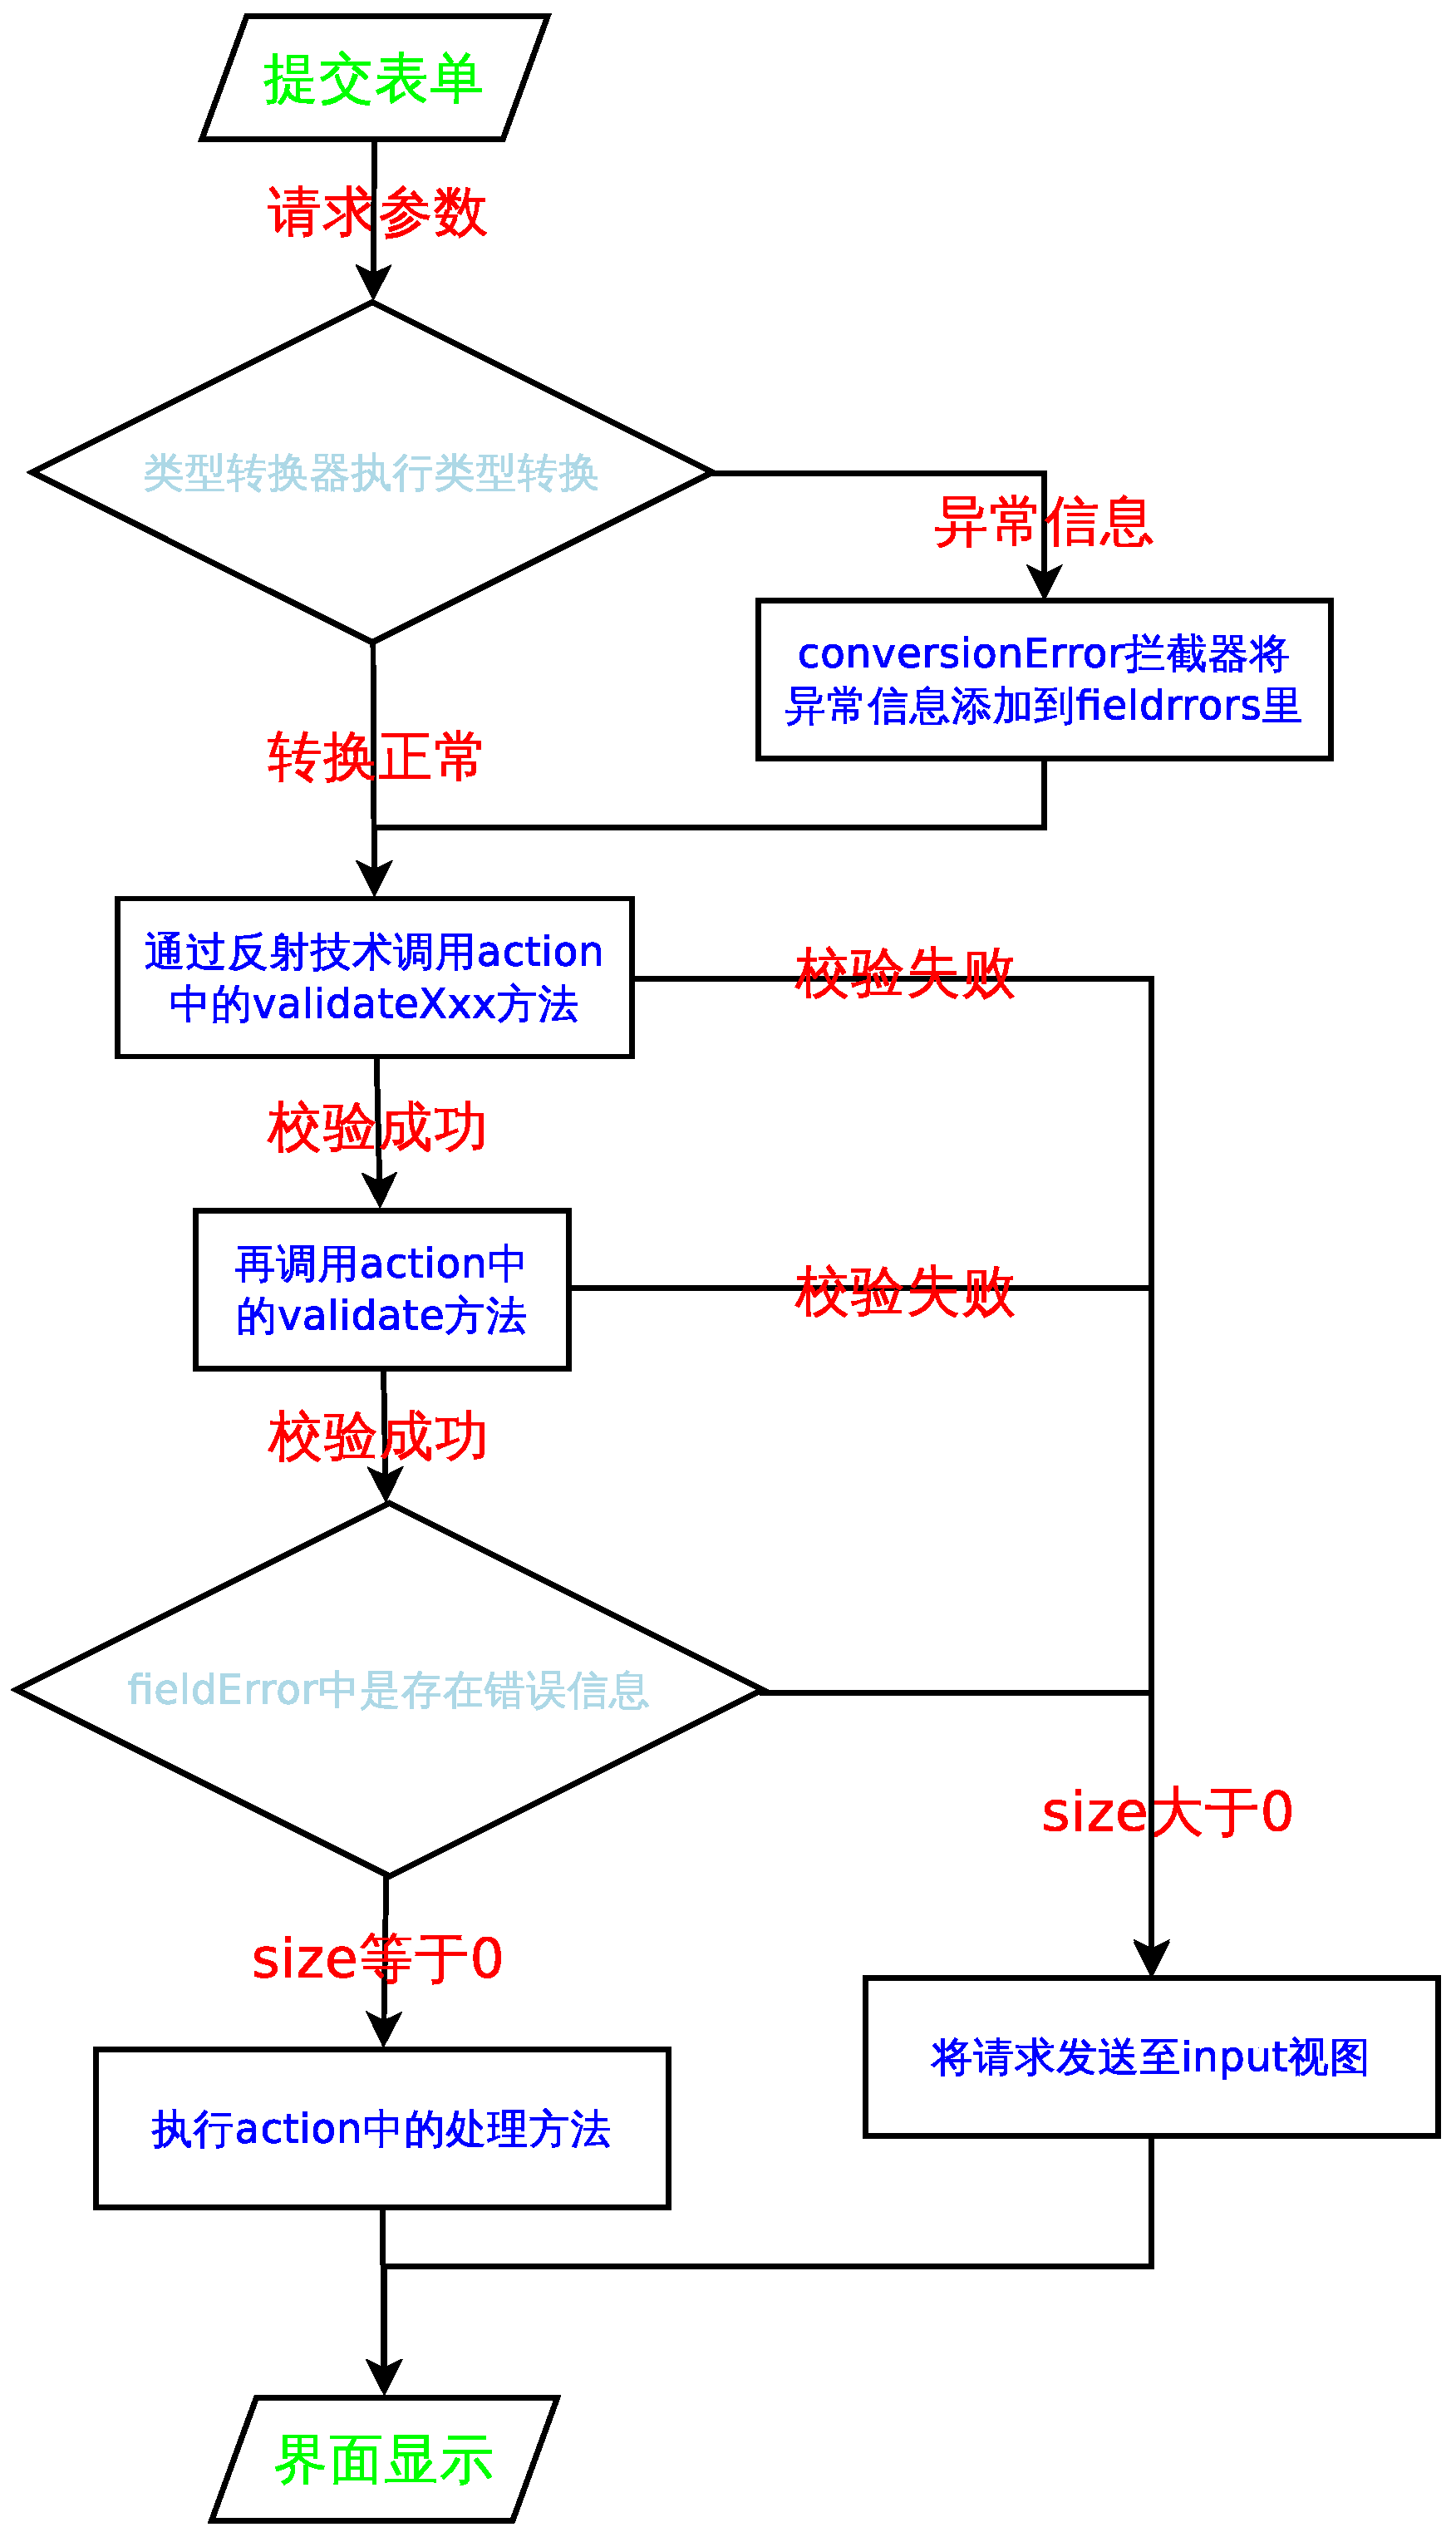
\includegraphics[scale=0.25]{figs/VALIDATE}
    \label{figs2:fig2}
\end{figure}

\end{itemize}

\item 基于XML配置方式实现
\begin{itemize}
\item 继承actionsupport类\\
com.opensymphony.xwork2.ActionSupport;
\item 新建校验文件,格式为ActionClassName-validation.xml,对所有action中方法有效的模板如下
\begin{lstlisting}[style=JAVA]
<?xml version="1.0" encoding="UTF-8"?>
<!DOCTYPE validators PUBLIC 
    "-//OpenSymphony Group//XWork Validator 1.0.3//EN"
    "http://www.opensymphony.com/xwork/xwork-validator-1.0.3.dtd">


<validators>
	<field name="username">
		<field-validator type="requiredstring">
			<param name="trim">true</param>
			<message>用户名不能为空!</message>
		</field-validator>
	</field>
	<field name="password">
		<field-validator type="requiredstring">
			<message>密码不能为空!</message>
		</field-validator>
		
		<field-validator type="stringlength">
			<!--指定user属性最小长度-->
        	<param name="minLength">4</param>
			<message>密码长度要大于4!</message>
		</field-validator>
	</field>
</validators>
\end{lstlisting}
\item 新建校验文件,格式为ActionClassName-actionName-validation.xml,对某个action方法有效的模板如下
\item 校验器种类
\begin{description}
\item[required] 必填校验器,要求filed的值不能为null
\item[requiredstring]	必填字符串校验器,要求field的值不能为null,并且长度大于0,
默认情况下会对字符串去前后空格
\item[stringlength]	字符串长度校验器,要求field的值必须在指定的范围内,否则校验失败,
minLength参数指定最小长度,maxLength参数指定最大长度,trim参数指定校验field之前是否去除
字符串前后的空格.
\item[regex]		正则表达式校验器,检查被校验的field是否匹配一个正则表达式,expression参数指定
正则表达式,caseSensitive参数指定进行正则表达式匹配时是否区分大小写,默认值为true.
\item[int]	整数校验器,要求field的整数值必须在指定范围内,min指定最小值,max指定最大值
\item[double]	双精度浮点数校验器,要求field的双精度浮点数必须在指定范围内,min指定最小值,
max指定最大值.
\item[fieldexpression]	字段OGNL表达式校验器,要求field满足一个ognl表达式,expression参数
指定ognl表达式.
\item[email]		邮件地址校验器,要求如果field的值非空,则必须是合法的邮件地址.
\item[url]	网址校验器,要求field的值非空,则必须是合法的url地址.
\item[date]	日期校验器,要求field的日期值必须在指定范围内,min指定最小值,max指定最大值.
\item[conversion]	转换校验器,指定在类型转换失败时,提示的错误信息.
\item[visitor]	用于校验action中的复合属性,它指定一个校验文件用于校验复合属性中的属性
\item[expression]	OGNL表达式校验器,expression参数指定ognl表达式,改逻辑表达式基于ValueStack
进行求值,返回true时,校验通过,否则不通过,该校验器不可用在字段校验器风格的配置中.
\end{description}

\item 验证失败后,请求转发给input视图
\begin{lstlisting}[style=JAVA]
<result name="input">/WEB-INF/login.jsp</result>
\end{lstlisting}
\item 显示\\
到input视图的界面用$<$s:fielderror$>$显示失败信息

\end{itemize}
\end{itemize}


\subsubsection{国际化}
不急


\subsection{OGNL表达式语言}


\subsection{JSTL}
\subsubsection{property标签}
\begin{description}
\item[default]	可选属性,如果需要输出的属性值为null,则显示该属性指定的值
\item[escape]	可选属性,指定是否格式化HTML代码
\item[value]		可选属性,指定需要输出的属性值,如果没有指定该属性,则默认输出ValueStack栈顶的值
\item[id]	可选属性,指定改元素的标识
\end{description}

\subsubsection{iterator标签}
iterator标签用于对集合进行迭代,这里的集合包含List,Set和数组.
\begin{description}
\item[value]		可选属性,指定被迭代的集合,如果没有设置该属性,则使用ValueStack栈顶的集合
\item[id]	可选属性,指定改元素的标识(已被标注为过时)
\item[status]	可选属性,该属性指定迭代时的iteratorStatus实例,该实例包含如下几个方法:
\begin{description}
\item[getCount]	返回当前迭代了几个元素
\item[getIndex]	返回当前迭代元素的索引
\item[isEven]	返回当前被迭代元素的索引是否是偶数
\item[isOdd]		返回当前被迭代元素的索引是否是奇数
\item[isFirst]	返回当前被迭代元素的索引是否是第一个元素
\item[isLast]	返回当前被迭代元素的索引是否是最后一个元素
\end{description}
\end{description}

\subsubsection{uri标签}
\begin{lstlisting}[style=JAVA]
<s:url action="passParameters" namespace="/path"><s:param name="id" value="11"/></s:url>
\end{lstlisting}
等价于\textcolor{red}{/struts2/path/passParameters.action?id=11}

\subsubsection{checkboxlist/select/radio标签}
\begin{enumerate}
\item 集合为list
\begin{lstlisting}[style=JAVA]
<s:checkboxlist name="list" list="{'java','net','ror','php'}" value="{'java','net'}"></s:checkboxlist>
\end{lstlisting}
等价与HTML的
\begin{lstlisting}[style=JAVA]
<input type="checkbox" name="list" value="java" id="list-1" checked="checked"/>
<label for="list-1" class="checkboxLabel">java</label>
<input type="checkbox" name="list" value="net" id="list-2" checked="checked"/>
<label for="list-2" class="checkboxLabel">net</label>
<input type="checkbox" name="list" value="ror" id="list-3"/>
<label for="list-3" class="checkboxLabel">ror</label>
<input type="checkbox" name="list" value="php" id="list-4"/>
<label for="list-4" class="checkboxLabel">php</label>
\end{lstlisting}
\item 集合为map
\begin{lstlisting}[style=JAVA]
<s:url action="passParameters" namespace="/path"><s:param name="id" value="11"/></s:url>
\end{lstlisting}
等价与HTML的
\begin{lstlisting}[style=JAVA]
<input type="checkbox" name="map" value="1" id="map-1" checked="checked"/>
<label for="map-1" class="checkboxLabel">javamap</label>
<input type="checkbox" name="map" value="2" id="map-2" checked="checked"/>
<label for="map-2" class="checkboxLabel">netmap</label>
<input type="checkbox" name="map" value="3" id="map-3" checked="checked"/>
<label for="map-3" class="checkboxLabel">rormap</label>
<input type="checkbox" name="map" value="4" id="map-4"/>
<label for="map-4" class="checkboxLabel">phpmap</label>
\end{lstlisting}
\end{enumerate}

\subsection{SSH整合开发}
\subsubsection{所需的jar包}
\begin{enumerate}
\item Struts2.1安装包
\begin{description}
\item[struts-core-2.x.x.jar]	Struts2框架的核心类库
\item[xwork-2.x.x.jar]	XWork类库,Struts 2在其上构建
\item[ognl-2.6.x.jar]	对象图导航语言,struts2框架通过其读写对象的属性
\item[freemarker-2.3.x.jar]	Struts2的UI标签的模板使用FreeMarker编写
\item[commons-fileupload-1.2.1.jar]	文件上传组件,2.1.6版本后必须加入此文件 
\item[struts2-spring-plugin-2.x.x.jar]	用于struts2集成spring的插件 
\end{description}

\item hibernate3.3核心安装包

\end{enumerate}



\subsection{FAQ}
\subsubsection{接受中文请求参数乱码问题}
出现这种情况,一般用户使用的是struts2.1.6版本或之前的,原因是struts2.1.6在获取并使用了请求参数后才调用
HttpServletRequest的setCharacterEncoding()方法进行编码设置,导致应用使用的就是乱码请求参数,这个bug
在struts2.1.8中已经被解决.\\
\underline{解决方法如下:}
新建一个Filter,把这个Filter放置在struts2的Filter之前,然后在doFilter()方法里添加以下代码:
\begin{lstlisting}[style=JAVA]
public void doFilter(...){
	HttpServletRequest req = (HttpServletRequest)request;
	req.setCharacterEncoding("UTF-8");	//replace UTF-8 with the encode you use
	filterchain.doFilter(request,response);
}
\end{lstlisting} 

\subsubsection{防止表单重复提交}`	
\begin{enumerate}
\item 在表单中加入<s:token/>标签(任意位置)
\item 在struts.xml配置中加入token拦截器和invalid.token结果.
\begin{lstlisting}[style=JAVA]
<action name="login_*" class="com.cm.LoginAction" method="{1}">
	<interceptor-ref name="defaultStack"/>
	<interceptor-ref name="token"/>
	<result name="sshow">/WEB-INF/sshow.jsp</result>
	<result name="invalid.token">/WEB-INF/slogin.jsp</result>
</action>
\end{lstlisting} 

\end{enumerate}